\documentclass{standalone}
\usepackage{tikz}
\usetikzlibrary{patterns, positioning}


\begin{document}
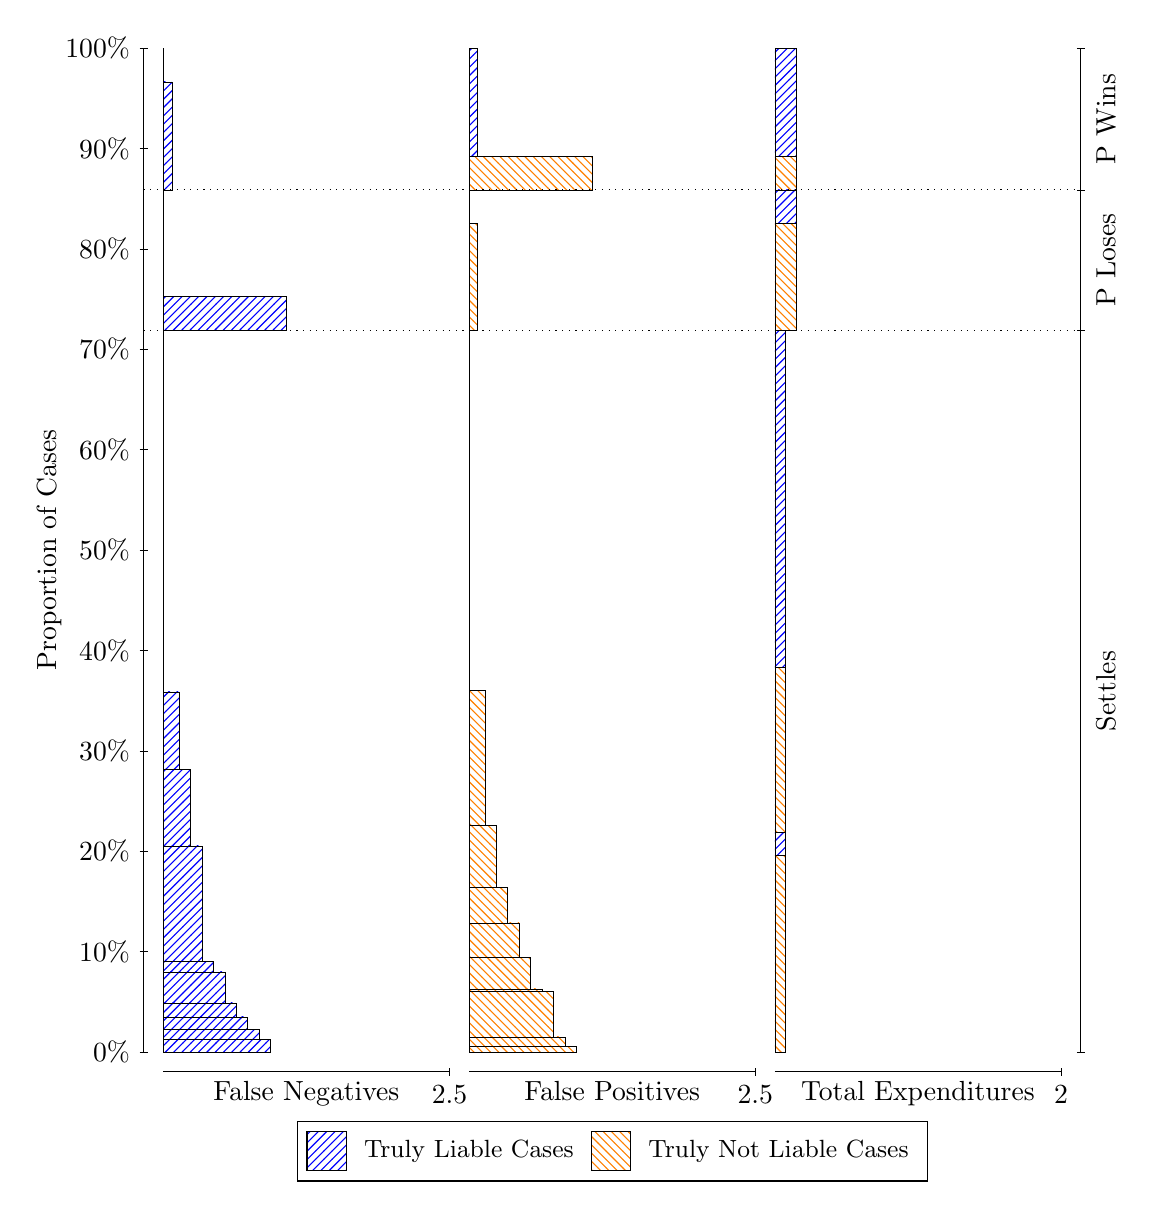
\begin{tikzpicture}
\draw[black, very thin] (1.5,1.75) -- (1.5,14.5);
\node[rotate=90, text=black, anchor=center] at (0.3, 8.125) {Proportion of Cases};
\draw[black, very thin] (1.45,1.75) -- (1.55,1.75);
\node[text=black, anchor=east] at (1.45, 1.75) {0\%};
\draw[black, very thin] (1.45,3.025) -- (1.55,3.025);
\node[text=black, anchor=east] at (1.45, 3.025) {10\%};
\draw[black, very thin] (1.45,4.3) -- (1.55,4.3);
\node[text=black, anchor=east] at (1.45, 4.3) {20\%};
\draw[black, very thin] (1.45,5.575) -- (1.55,5.575);
\node[text=black, anchor=east] at (1.45, 5.575) {30\%};
\draw[black, very thin] (1.45,6.85) -- (1.55,6.85);
\node[text=black, anchor=east] at (1.45, 6.85) {40\%};
\draw[black, very thin] (1.45,8.125) -- (1.55,8.125);
\node[text=black, anchor=east] at (1.45, 8.125) {50\%};
\draw[black, very thin] (1.45,9.4) -- (1.55,9.4);
\node[text=black, anchor=east] at (1.45, 9.4) {60\%};
\draw[black, very thin] (1.45,10.675) -- (1.55,10.675);
\node[text=black, anchor=east] at (1.45, 10.675) {70\%};
\draw[black, very thin] (1.45,11.95) -- (1.55,11.95);
\node[text=black, anchor=east] at (1.45, 11.95) {80\%};
\draw[black, very thin] (1.45,13.225) -- (1.55,13.225);
\node[text=black, anchor=east] at (1.45, 13.225) {90\%};
\draw[black, very thin] (1.45,14.5) -- (1.55,14.5);
\node[text=black, anchor=east] at (1.45, 14.5) {100\%};

\draw[black, very thin] (13.4,1.75) -- (13.4,14.5);
\draw[black, very thin] (13.35,1.75) -- (13.45,1.75);
\node[anchor=west] at (13.35, 1.75) {};
\draw[black, very thin] (13.35,10.918) -- (13.45,10.918);
\node[anchor=west] at (13.35, 10.918) {};
\draw[black, very thin] (13.35,12.698) -- (13.45,12.698);
\node[anchor=west] at (13.35, 12.698) {};
\draw[black, very thin] (13.35,14.5) -- (13.45,14.5);
\node[anchor=west] at (13.35, 14.5) {};

\draw[black, very thin, pattern color=blue, pattern=north east lines] (1.75,1.75) rectangle (3.1125,1.9083);
\draw[black, very thin, pattern color=blue, pattern=north east lines] (1.75,1.9083) rectangle (2.9672,2.0379);
\draw[black, very thin, pattern color=blue, pattern=north east lines] (1.75,2.0379) rectangle (2.8218,2.1969);
\draw[black, very thin, pattern color=blue, pattern=north east lines] (1.75,2.1969) rectangle (2.6765,2.3743);
\draw[black, very thin, pattern color=blue, pattern=north east lines] (1.75,2.3743) rectangle (2.5312,2.7685);
\draw[black, very thin, pattern color=blue, pattern=north east lines] (1.75,2.7685) rectangle (2.3858,2.8995);
\draw[black, very thin, pattern color=blue, pattern=north east lines] (1.75,2.8995) rectangle (2.2405,4.3659);
\draw[black, very thin, pattern color=blue, pattern=north east lines] (1.75,4.3659) rectangle (2.0952,5.3353);
\draw[black, very thin, pattern color=blue, pattern=north east lines] (1.75,5.3353) rectangle (1.9498,6.3234);
\draw[black, very thin, pattern color=orange, pattern=north west lines] (1.75,6.3234) rectangle (1.75,10.918);
\draw[black, very thin, pattern color=blue, pattern=north east lines] (1.75,10.918) rectangle (3.3123,11.347);
\draw[black, very thin, pattern color=orange, pattern=north west lines] (1.75,11.347) rectangle (1.75,12.698);
\draw[black, very thin, pattern color=blue, pattern=north east lines] (1.75,12.698) rectangle (1.859,14.071);
\draw[black, very thin, pattern color=orange, pattern=north west lines] (1.75,14.071) rectangle (1.75,14.5);
\draw[black, very thin, pattern color=orange, pattern=north west lines] (5.6333,1.75) rectangle (6.9958,1.817);
\draw[black, very thin, pattern color=orange, pattern=north west lines] (5.6333,1.817) rectangle (6.8505,1.9425);
\draw[black, very thin, pattern color=orange, pattern=north west lines] (5.6333,1.9425) rectangle (6.7052,2.5154);
\draw[black, very thin, pattern color=orange, pattern=north west lines] (5.6333,2.5154) rectangle (6.5598,2.5522);
\draw[black, very thin, pattern color=orange, pattern=north west lines] (5.6333,2.5522) rectangle (6.4145,2.9546);
\draw[black, very thin, pattern color=orange, pattern=north west lines] (5.6333,2.9546) rectangle (6.2692,3.3891);
\draw[black, very thin, pattern color=orange, pattern=north west lines] (5.6333,3.3891) rectangle (6.1238,3.8431);
\draw[black, very thin, pattern color=orange, pattern=north west lines] (5.6333,3.8431) rectangle (5.9785,4.6245);
\draw[black, very thin, pattern color=orange, pattern=north west lines] (5.6333,4.6245) rectangle (5.8332,6.3445);
\draw[black, very thin, pattern color=blue, pattern=north east lines] (5.6333,6.3445) rectangle (5.6333,10.918);
\draw[black, very thin, pattern color=orange, pattern=north west lines] (5.6333,10.918) rectangle (5.7423,12.269);
\draw[black, very thin, pattern color=blue, pattern=north east lines] (5.6333,12.269) rectangle (5.6333,12.698);
\draw[black, very thin, pattern color=orange, pattern=north west lines] (5.6333,12.698) rectangle (7.1957,13.127);
\draw[black, very thin, pattern color=blue, pattern=north east lines] (5.6333,13.127) rectangle (5.7423,14.5);
\draw[black, very thin, pattern color=orange, pattern=north west lines] (9.5167,1.75) rectangle (9.6529,4.2514);
\draw[black, very thin, pattern color=blue, pattern=north east lines] (9.5167,4.2514) rectangle (9.6529,4.5393);
\draw[black, very thin, pattern color=orange, pattern=north west lines] (9.5167,4.5393) rectangle (9.6529,6.6324);
\draw[black, very thin, pattern color=blue, pattern=north east lines] (9.5167,6.6324) rectangle (9.6529,10.918);
\draw[black, very thin, pattern color=orange, pattern=north west lines] (9.5167,10.918) rectangle (9.7892,12.269);
\draw[black, very thin, pattern color=blue, pattern=north east lines] (9.5167,12.269) rectangle (9.7892,12.698);
\draw[black, very thin, pattern color=orange, pattern=north west lines] (9.5167,12.698) rectangle (9.7892,13.127);
\draw[black, very thin, pattern color=blue, pattern=north east lines] (9.5167,13.127) rectangle (9.7892,14.5);
\draw[black, dotted] (1.5,10.918) -- (13.4,10.918);
\draw[black, dotted] (1.5,12.698) -- (13.4,12.698);
\draw[black, very thin] (1.75,1.5) -- (5.3833,1.5);
\node[text=black, anchor=north] at (3.5667, 1.5) {False Negatives};
\draw[black, very thin] (5.3833,1.45) -- (5.3833,1.55);
\node[text=black, anchor=north] at (5.3833, 1.45) {2.5};

\draw[black, very thin] (5.6333,1.5) -- (9.2667,1.5);
\node[text=black, anchor=north] at (7.45, 1.5) {False Positives};
\draw[black, very thin] (9.2667,1.45) -- (9.2667,1.55);
\node[text=black, anchor=north] at (9.2667, 1.45) {2.5};

\draw[black, very thin] (9.5167,1.5) -- (13.15,1.5);
\node[text=black, anchor=north] at (11.333, 1.5) {Total Expenditures};
\draw[black, very thin] (13.15,1.45) -- (13.15,1.55);
\node[text=black, anchor=north] at (13.15, 1.45) {2};

\node[text=black, centered, rotate=90] at (13.72, 6.3339) {Settles};
\node[text=black, centered, rotate=90] at (13.72, 11.808) {P Loses};
\node[text=black, centered, rotate=90] at (13.72, 13.599) {P Wins};

\draw (7.449999999999999,1.5) node[draw=none] (baseCoordinate) {};
\begin{scope}[align=center]
        \matrix[scale=0.5, draw=black, below=0.5cm of baseCoordinate, nodes={draw}, column sep=0.1cm]{
            \node[rectangle, draw, minimum width=0.5cm, minimum height=0.5cm, pattern color=blue, pattern=north east lines] {}; &
            \node[draw=none, font=\small, text=black] (B) {Truly Liable Cases}; &
            \node[rectangle, draw, minimum width=0.5cm, minimum height=0.5cm, pattern color=orange, pattern=north west lines] {}; &
            \node[draw=none, font=\small, text=black] (B) {Truly Not Liable Cases}; \\
            };
\end{scope}

\end{tikzpicture}
\end{document}